% Multiple Choice Question 16 to 17 (2 questions)

% \par\noindent\rule{0.75\textwidth}{0.5pt} 
\textbf{See the instruction for questions \inteval{\value{question}+1} to \inteval{\value{question}+2}.} 

\begin{center}
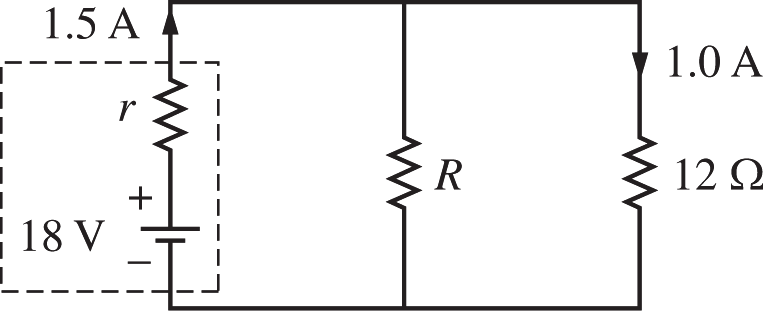
\includegraphics[scale=0.3]{images/img-008-009.png}
\end{center}

Two resistors of resistances $R$ and $12 \unit{\Omega}$ are connected to a battery of emf $18 \unit{V}$, as shown in the figure above. The battery has an internal resistance of $r$. The current in the battery is $1.5 \unit{A}$, and the current in the $12 \unit{\Omega}$ resistor is $1.0 \unit{A}$.

\begin{questions}
\setcounter{question}{15}

% Multiple Choice Question 16
\question
What is the resistance $R$?

\begin{oneparchoices}
    \choice $7.2 \unit{\Omega}$
    \choice $12 \unit{\Omega}$
    \choice $18 \unit{\Omega}$
    \choice $24 \unit{\Omega}$
    \choice $45 \unit{\Omega}$
\end{oneparchoices}

% Multiple Choice Question 17
\question
What is the internal resistance of the battery?

\begin{oneparchoices}
    \choice $4.0 \unit{\Omega}$
    \choice $6.0 \unit{\Omega}$
    \choice $12 \unit{\Omega}$
    \choice $18 \unit{\Omega}$
    \choice $36 \unit{\Omega}$
\end{oneparchoices}

\end{questions}
